%\documentclass{beamer}
\documentclass[aspectratio=169]{beamer}
\usetheme{Boadilla}

%\usetheme{Warsaw}
%\setbeamercovered{transparent}
\beamertemplatetransparentcoveredhigh
\usepackage[portuges]{babel}
\usepackage[latin1]{inputenc}
\usepackage{lmodern}
\usepackage[T1]{fontenc}
\usepackage{hyperref} 
\usepackage[portuguese, linesnumbered, vlined, titlenumbered, ruled]{algorithm2e}

\newcommand{\eng}[1]{\textsl{#1}}
\newcommand{\cod}[1]{\texttt{#1}}

\title[Apresenta��o]{Curso Intelig�ncia Artificial: do Zero ao Infinito}
\author[Frederico Oliveira]{Modelos SSD}
\institute[UFMT]{Universidade Federal de Mato Grosso}
\date{}
%\titlegraphic{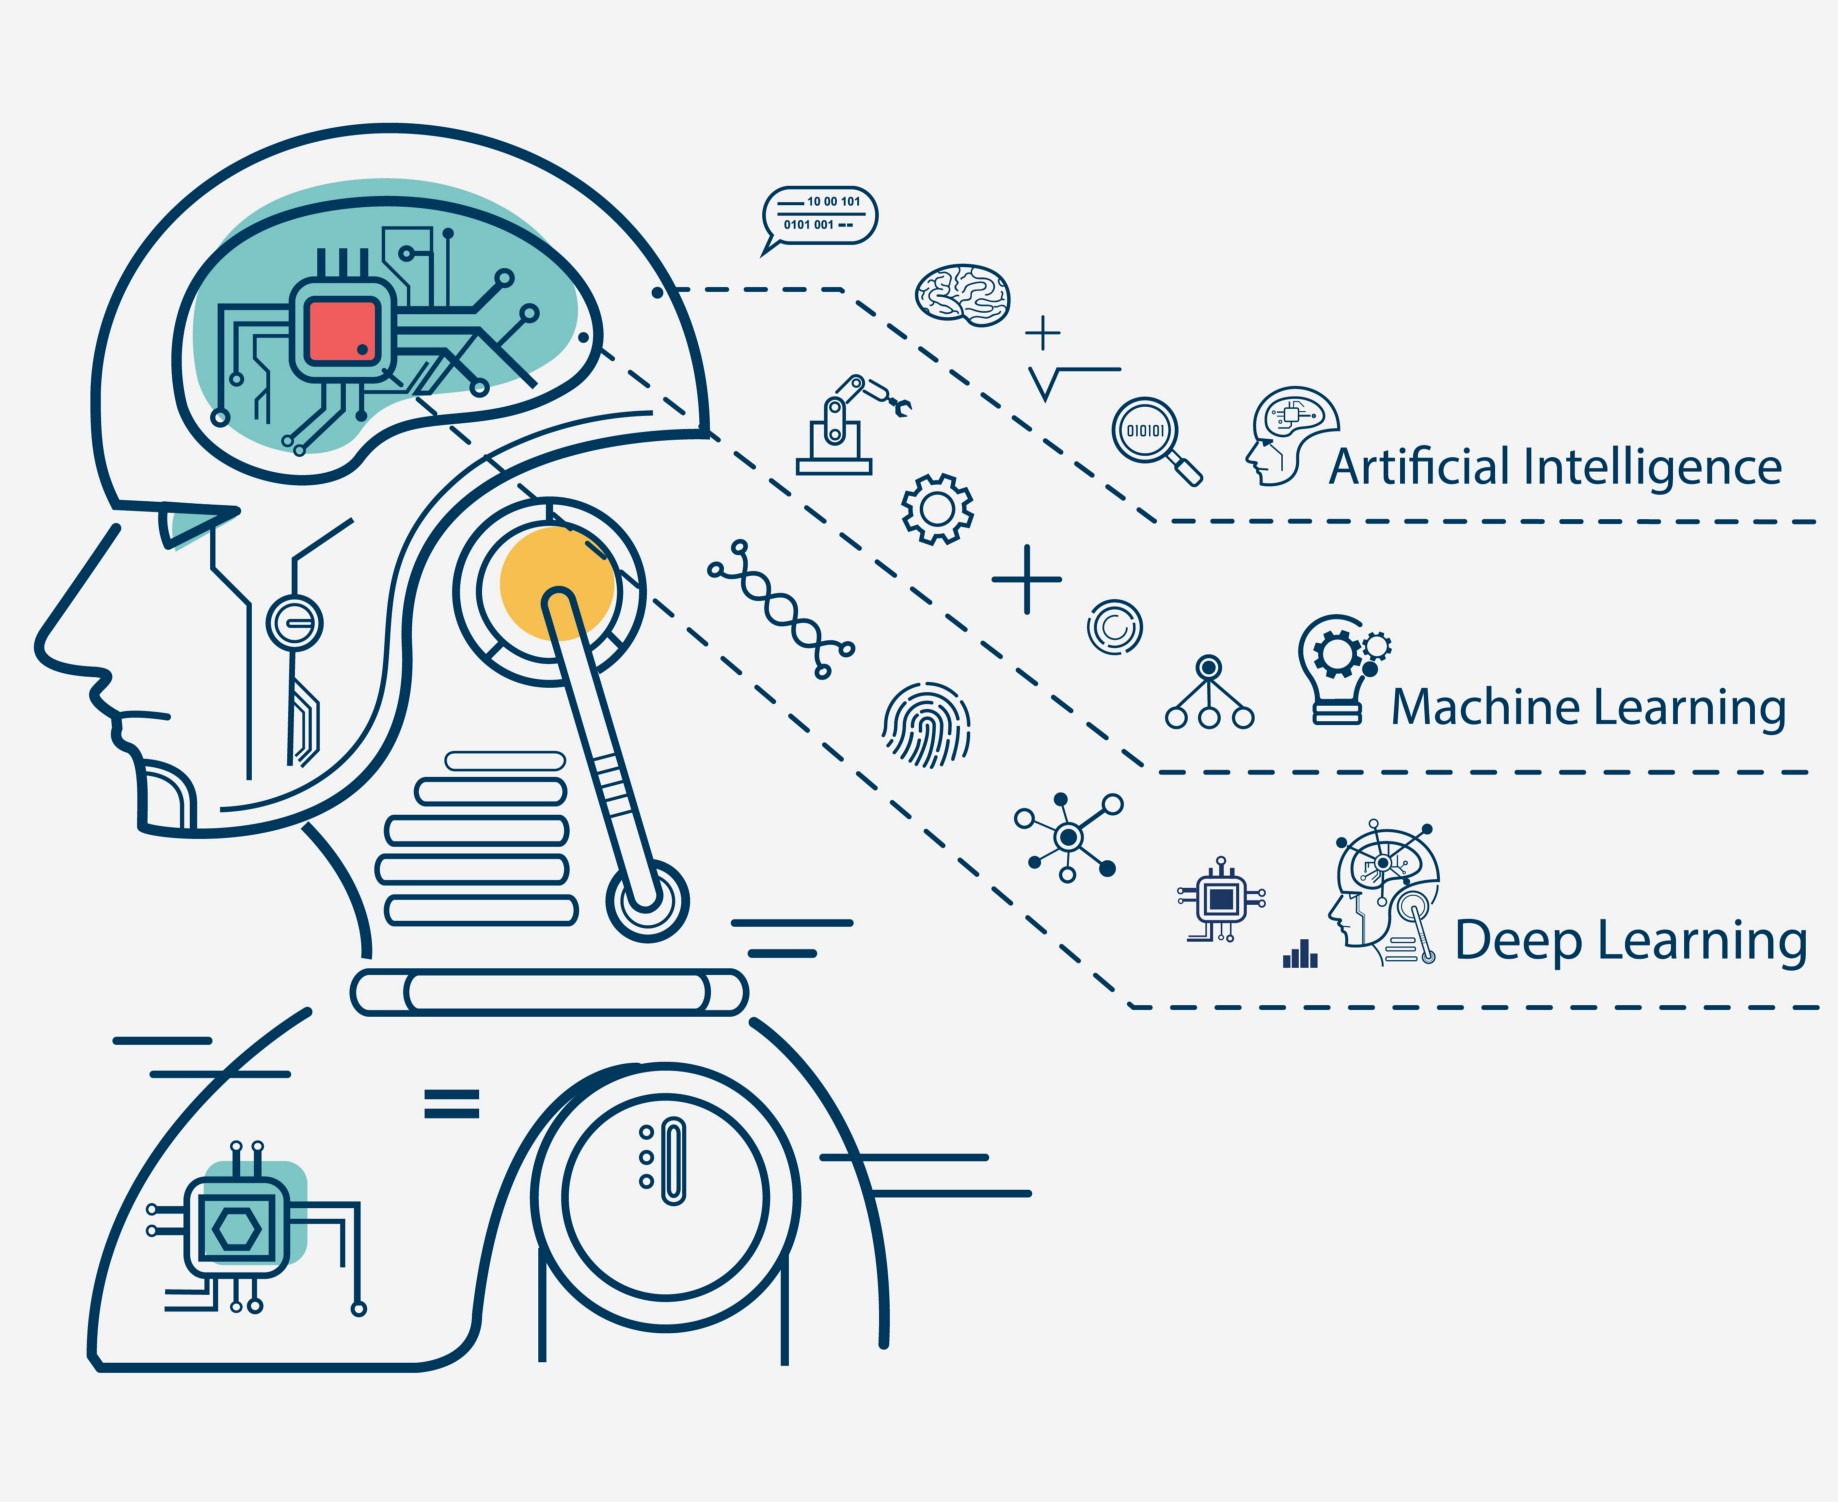
\includegraphics[width=\textwidth,height=.5\textheight]{imgs/intro.jpeg}}
%\usebackgroundtemplate{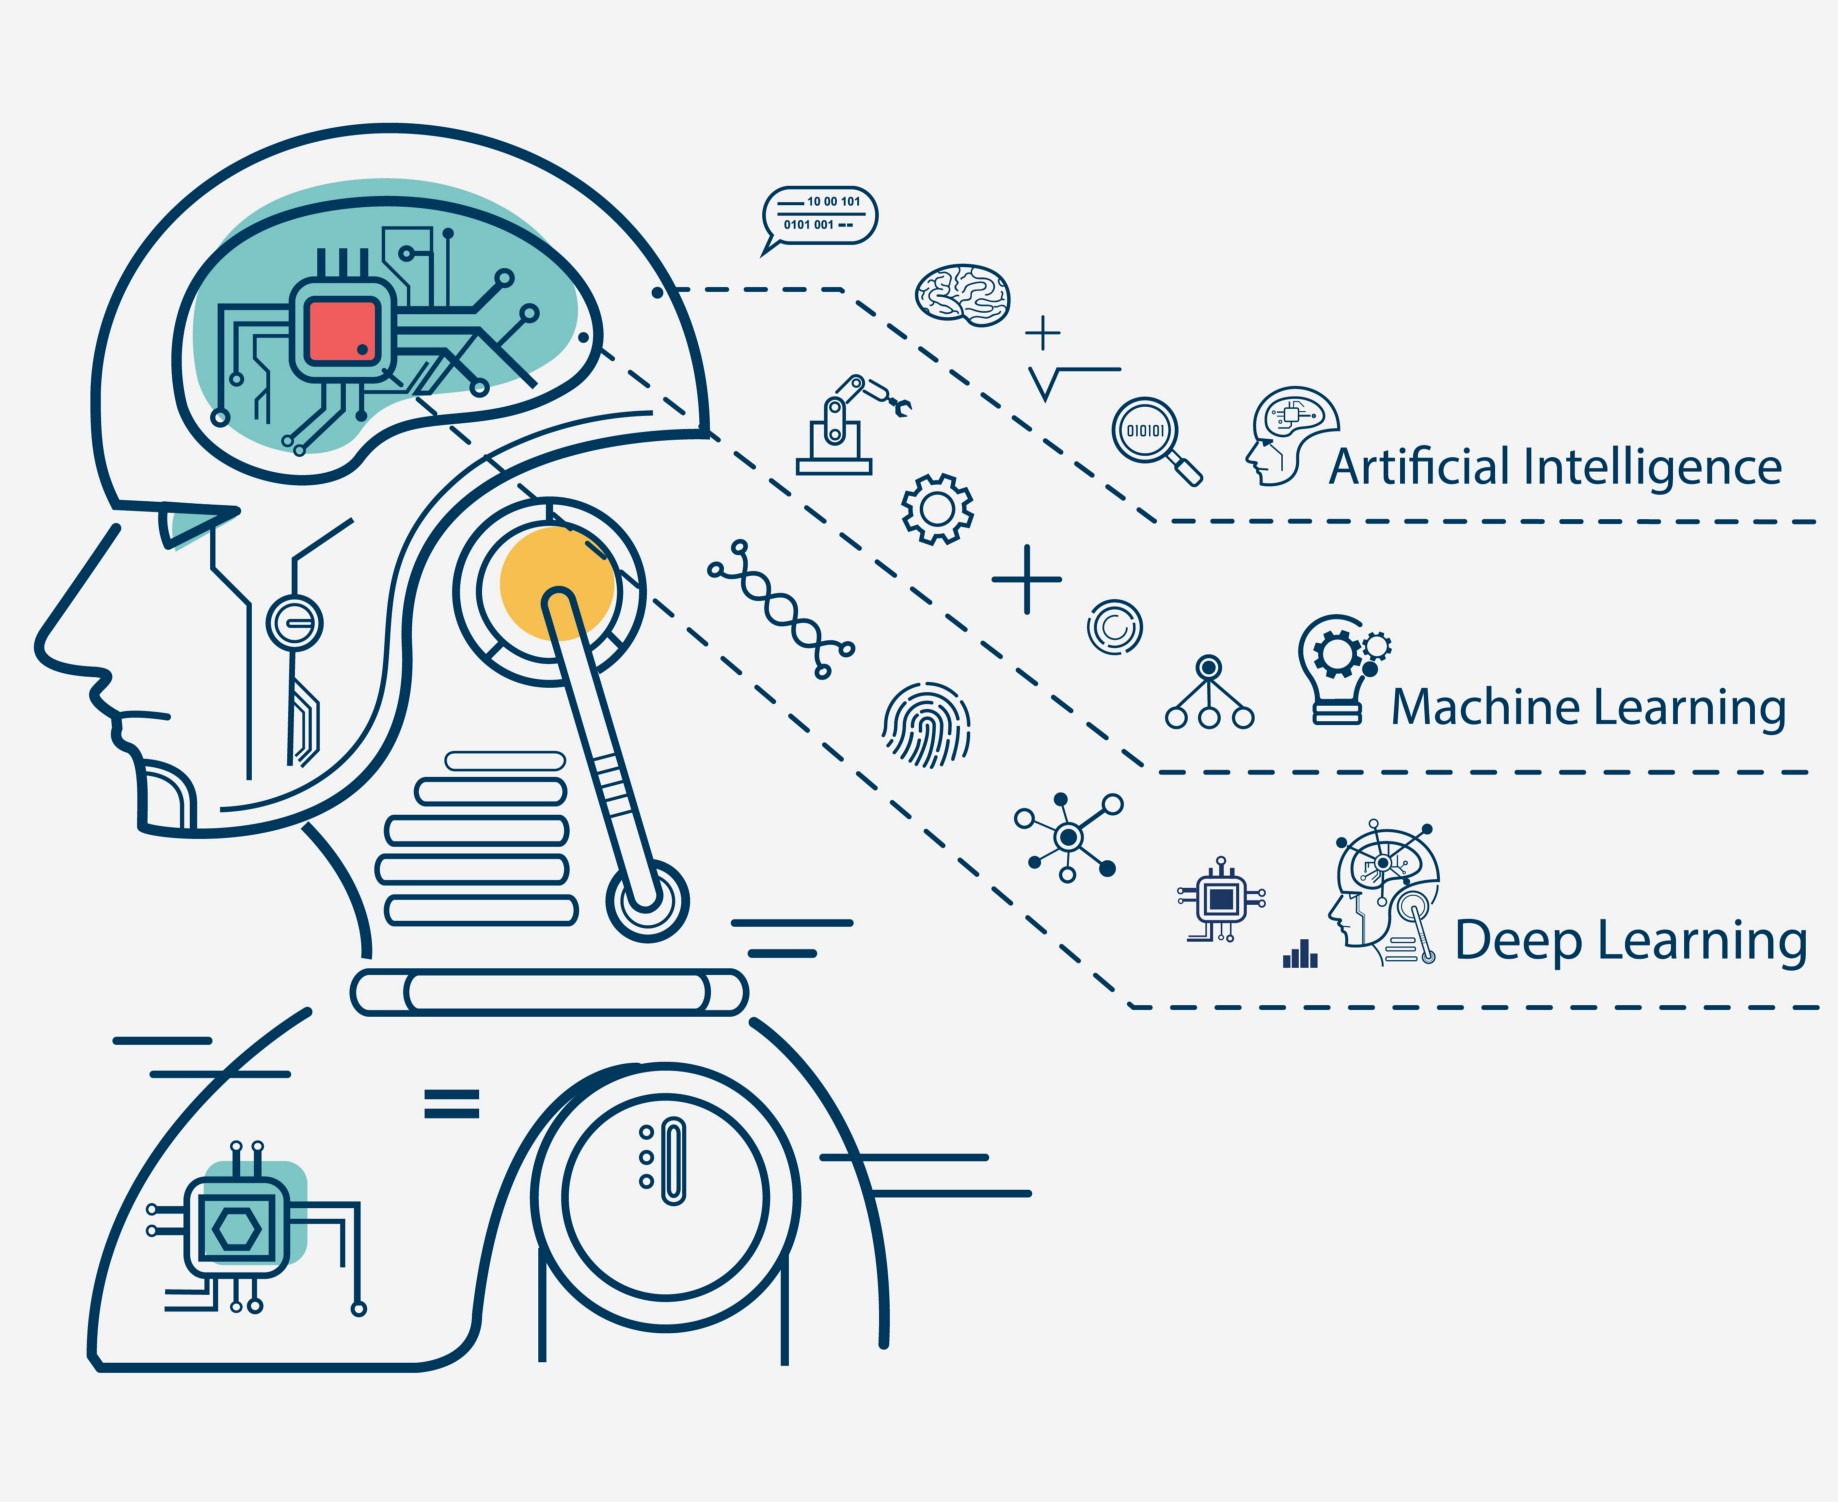
\includegraphics[width=\paperwidth]{imgs/intro.jpeg}}
\begin{document}

\begin{frame}[plain]
  \titlepage
\end{frame}

%%%%%%%%%%%%%%%%%%%%%%%%%%%%%%%%%%%%%%%%%%%%%%%%%%%%%%%%%%%%%%%%%%%%%%%%%%%%%%%%%%%%%%%%%%%%%%%%%%%%%%%%%%%%%%%%
%\section*{Roteiro}
%%%%%%%%%%%%%%%%%%%%%%%%%%%%%%%%%%%%%%%%%%%%%%%%%%%%%%%%%%%%%%%%%%%%%%%%%%%%%%%%%%%%%%%%%%%%%%%%%%%%%%%%%%%%%%%%

\begin{frame}
  \frametitle{Agenda}
  \tableofcontents
\end{frame}

%%%%%%%%%%%%%%%%%%%%%%%%%%%%%%%%%%%%%%%%%%%%%%%%%%%%%%%%%%%%%%%%%%%%%%%%%%%%%%%%%%%%%%%%%%%%%%%%%%%%%%%%%%%%%%%%
\section{Introdu��o}
%%%%%%%%%%%%%%%%%%%%%%%%%%%%%%%%%%%%%%%%%%%%%%%%%%%%%%%%%%%%%%%%%%%%%%%%%%%%%%%%%%%%%%%%%%%%%%%%%%%%%%%%%%%%%%%%

\begin{frame}{Detec��o de Objetos}{Arquiteturas}
\begin{itemize}
\item {\bf R-CNN} (Regions with Convolutional Network)
\item {\bf Fast-RCNN}
\item {\bf Faster-RCNN}
\item {\bf MobileNet}
\end{itemize}
\end{frame}

%%%%%%%%%%%%%%%%%%%%%%%%%%%%%%%%%%%%%%%%%%%%%%%%%%%%%%%%%%%%%%%%%%%%%%%%%%%%%%%%%%%%%%%%%%%%%%%%%%%%%%%%%%%%%%%%
\section{SSD - Single Shot MultiBox Detector}
%%%%%%%%%%%%%%%%%%%%%%%%%%%%%%%%%%%%%%%%%%%%%%%%%%%%%%%%%%%%%%%%%%%%%%%%%%%%%%%%%%%%%%%%%%%%%%%%%%%%%%%%%%%%%%%%

\begin{frame}{SSD - Single Shot MultiBox Detector}
\begin{itemize}
\item O modelo SSD foi apresentado em 2016 e utiliza a VGG16 para extra��o de um {\it features map}.
\item Nesse modelo, elimina-se a necessidade de uma rede para detec��o das {\it Region Proposals}.
\item Utiliza uma s�rie de camadas convolucionais $3 \times 3$ para avaliar os {\it bboxes}.
\item Encontra-se as {\it bboxes} realizando classifica��o em todas as posi��es da imagem, utilizando diferentes formas e escalas.
\end{itemize}

\vspace{1cm}
\tiny{Paper: \href{https://arxiv.org/pdf/1512.02325.pdf}{SSD: Single Shot MultiBox Detector}}
\end{frame}

%%%%%%%%%%%%%%%%%%%%%%%%%%%%%%%%%%%%%%%%%%%%%%%%%%%%%%%%%%%%%%%%%%%%%%%%%%%%%%%%%%%%%%%%%%%%%%%%%%%%%%%%%%%%%%%%

\begin{frame}{SSD - Single Shot MultiBox Detector}
O nome do modelo explica sua arquitetura:
\begin{itemize}
\item {\bf Single Shot}: significa que as etapas de localiza��o e classifica��o de objetos s�o feitos em uma �nica etapa;
\item {\bf Multibox}: � o nome da t�cnica de regres	s�o para gera��o dos {\it bboxes}, proposta por Szegedy;
\item {\bf Detector}: a rede � um detector de objetos que tamb�m os classifica.
\end{itemize}

\vspace{1cm}
\tiny{Fonte: \href{https://towardsdatascience.com/understanding-ssd-multibox-real-time-object-detection-in-deep-learning-495ef744fab}{Understanding SSD MultiBox - Real-Time Object Detection In Deep Learning}}

\tiny{Paper Szegedy: \href{https://arxiv.org/pdf/1412.1441.pdf}{Scalable, High-Quality Object Detection}}
\end{frame}

%%%%%%%%%%%%%%%%%%%%%%%%%%%%%%%%%%%%%%%%%%%%%%%%%%%%%%%%%%%%%%%%%%%%%%%%%%%%%%%%%%%%%%%%%%%%%%%%%%%%%%%%%%%%%%%%%

\begin{frame}{SSD - Single Shot MultiBox Detector}
\begin{figure}[h]
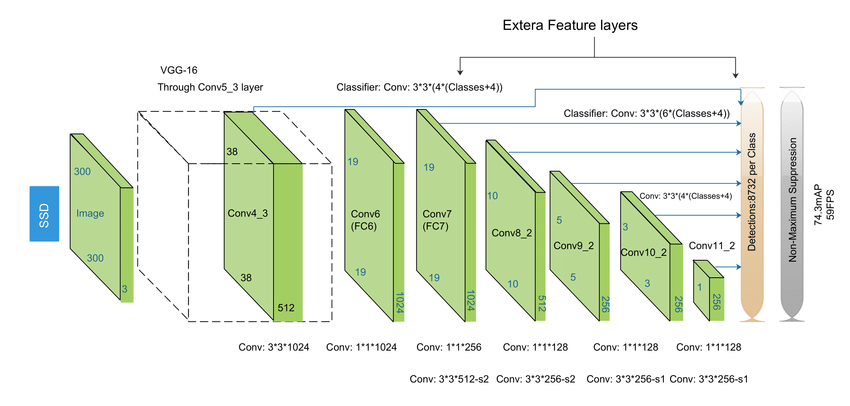
\includegraphics[width=12cm]{imgs/ssd_architecture.png}
\end{figure}

\vspace{1cm}
\tiny{Fonte: \href{https://www.researchgate.net/figure/Single-Shot-Multi-Box-Detector-SSD-architecture-47_fig4_340654462}{https://www.researchgate.net/figure/Single-Shot-Multi-Box-Detector-SSD-architecture}}
\end{frame}

%%%%%%%%%%%%%%%%%%%%%%%%%%%%%%%%%%%%%%%%%%%%%%%%%%%%%%%%%%%%%%%%%%%%%%%%%%%%%%%%%%%%%%%%%%%%%%%%%%%%%%%%%%%%%%%%%

\begin{frame}{SSD - Single Shot MultiBox Detector}{Architecture}
\begin{figure}[h]
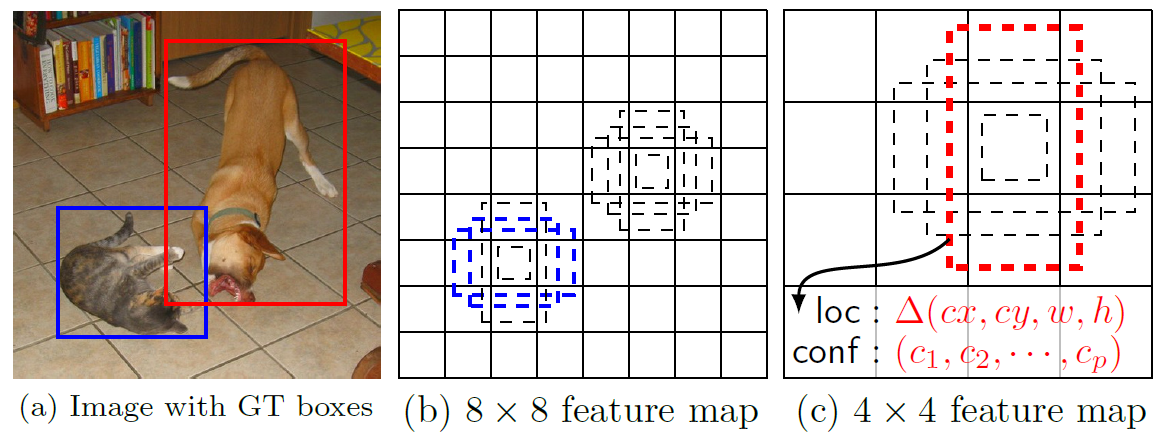
\includegraphics[width=10cm]{imgs/ssd_multibox_detector.png}
\end{figure}

\vspace{1cm}
\tiny{Paper: \href{https://arxiv.org/pdf/1512.02325.pdf}{SSD: Single Shot MultiBox Detector}}
\end{frame}

%%%%%%%%%%%%%%%%%%%%%%%%%%%%%%%%%%%%%%%%%%%%%%%%%%%%%%%%%%%%%%%%%%%%%%%%%%%%%%%%%%%%%%%%%%%%%%%%%%%%%%%%%%%%%%%%
\section{Pr�ximas Arquiteturas}
%%%%%%%%%%%%%%%%%%%%%%%%%%%%%%%%%%%%%%%%%%%%%%%%%%%%%%%%%%%%%%%%%%%%%%%%%%%%%%%%%%%%%%%%%%%%%%%%%%%%%%%%%%%%%%%%

\begin{frame}{Detec��o de Objetos}{Pr�ximas Arquiteturas}
\begin{itemize}
\item{\bf YOLO}
\item {\bf RetinaNet} 
\item {\bf SqueezeDet}
\end{itemize}
\end{frame}


%%%%%%%%%%%%%%%%%%%%%%%%%%%%%%%%%%%%%%%%%%%%%%%%%%%%%%%%%%%%%%%%%%%%%%%%%%%%%%%%%%%%%%%%%%%%%%%%%%%%%%%%%%%%%%%%

\begin{frame}{Referencias}
\begin{itemize}
\item Paper - SSD: Single Shot MultiBox Detector
  \begin{itemize}
  \item \url{https://arxiv.org/pdf/1512.02325.pdf}
  \end{itemize}  
\item SSD object detection: Single Shot MultiBox Detector for real-time processing
  \begin{itemize}
  \item \url{https://jonathan-hui.medium.com/ssd-object-detection-single-shot-multibox-detector-for-real-time-processing-9bd8deac0e06}
  \end{itemize}  
\item Understanding SSD MultiBox - Real-Time Object Detection In Deep Learning
  \begin{itemize}
  \item \url{https://towardsdatascience.com/understanding-ssd-multibox-real-time-object-detection-in-deep-learning-495ef744fab}
  \end{itemize}  
\item Livro: Dive Into Deep Learning - Single Shot Multibox Detection
  \begin{itemize}
  \item \url{https://d2l.ai/chapter_computer-vision/ssd.html}
  \end{itemize}    
  
\end{itemize}
\end{frame}

%%%%%%%%%%%%%%%%%%%%%%%%%%%%%%%%%%%%%%%%%%%%%%%%%%%%%%%%%%%%%%%%%%%%%%%%%%%%%%%%%%%%%%%%%%%%%%%%%%%%%%%%%%%%%%%%

\begin{frame}[plain]
  \titlepage
\end{frame}


\end{document}
